\chapter{The Electronic Basis for Memory}

In our studies of computer science at the University of Alberta, we rarely mention the underlying electronics that form the basis of electronic logic systems, and hence computers. Despite our high level abstractions away from silicon when learning how to write code, a robust understanding of the underlying principles of computing systems encourages students to think about the physical limitations of our current systems and why we design our systems as we do. This section will scratch the surface of electrical engineering and provide the reader with the essential background to determine why certain artifacts, like CAS latency, appear in the analysis of the memory subsystem.

\section{The Transistor and Capacitor}

When studying memory systems, there are two fundamental structures we need to understand: the transistor and the capacitor. For our purposes it suffices to think of the capacitor as a battery and the transistor as a switch, the following section is an elaboration on those simplifications.

\begin{figure}
  \centering
  \begin{tikzpicture}
    % Draw the capacitor
    \draw (-2,1) -- (0,1) to[capacitor, l=$C$] (2,1) -- (4,1);
    
    % Add the image next to the capacitor
    \node at (3,-1) {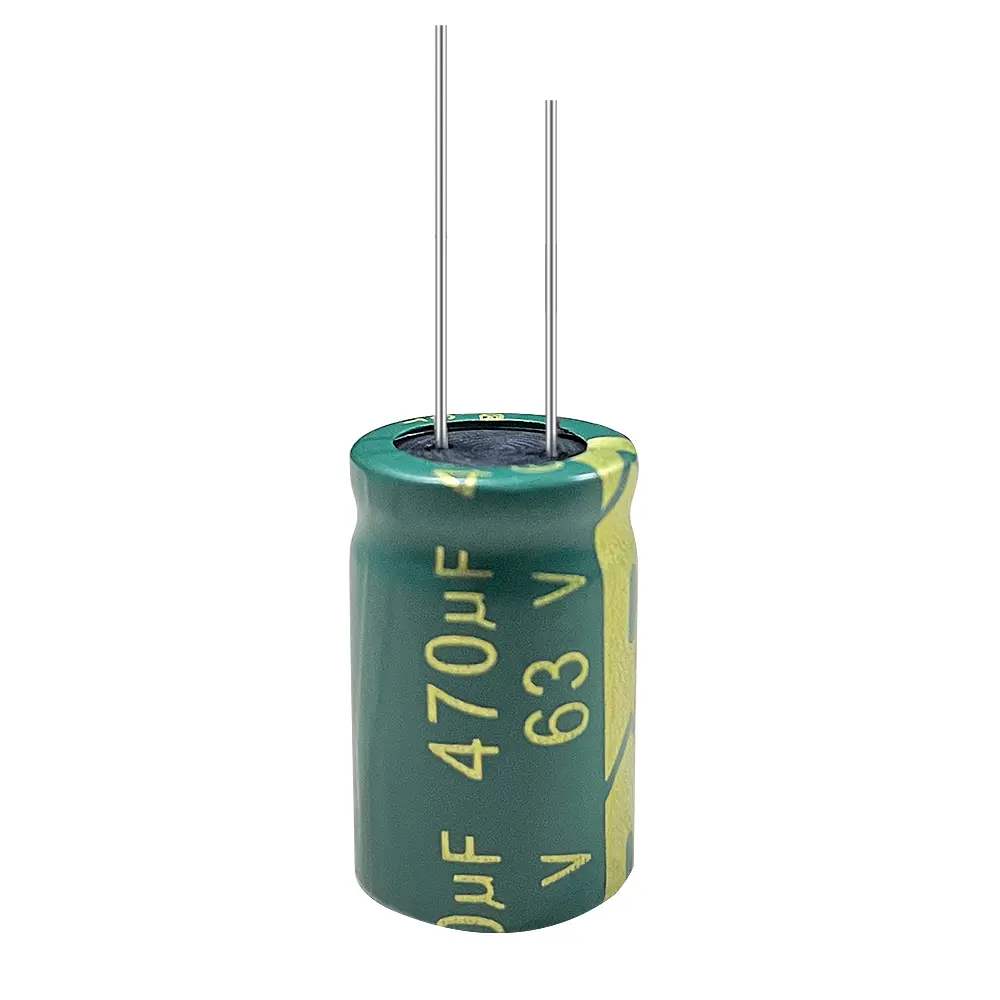
\includegraphics[width=2cm]{assets/capacitor.png}};
  \end{tikzpicture}
  \caption{A Capacitor.}
\end{figure}
Beginning with the capacitor, a capacitor accumulates and stores charge as the buildup of a potential difference between two surfaces insulated from each other~\cite{wiki:capacitor}. They serve as the physical storage for a single bit in conjunction with a transistor and a ground. Charging a capacitor is a relatively slow operation (relative to the modification of an SRAM cell, as we will discuss in a moment), but the die area of a capacitor and single transistor is significantly less than the die area required for a single cell of SRAM (6 transistors), thus allowing us to produce large capacity DRAM cheaply.

\begin{figure}
  \centering
  \begin{tikzpicture}
    % Draw the NMOS transistor
    \draw (0,0) node[nmos, anchor=D] (transistor) {};

    % Connect and label the source
    \draw (transistor.S) -- ++(0,-1) node[below] {Source};

    % Connect and label the drain
    \draw (transistor.D) -- ++(0,1) node[above] {Drain};

    % Connect and label the gate
    \draw (transistor.G) -- ++(-1,0) node[left] {Gate};

    % Add the image next to the transistor
    \node at (3,0) {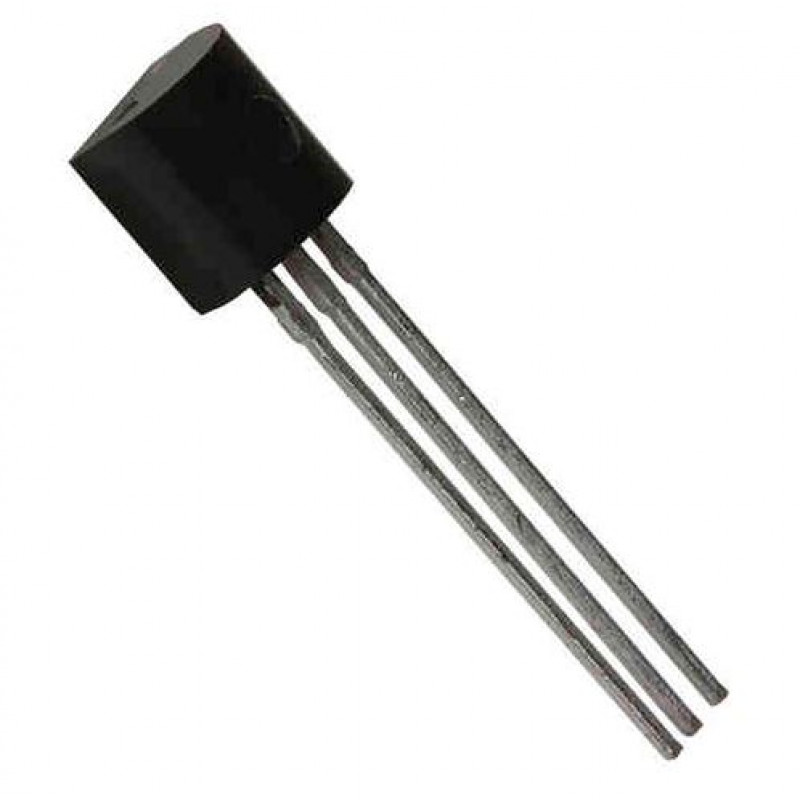
\includegraphics[width=2cm]{assets/transistor.jpg}};
  \end{tikzpicture}
  \caption{A Transistor.}
\end{figure}

The transistor is our next target of study. Simplistically, the transistor is a switch. It consists of three connections: the source, the gate and the drain. The gate serves as the switching mechanism: when we apply current to the gate, current can flow freely between the source and the drain. When no current is applied to the gate, no electricity can flow from the source and drain. The transistors used in hobby projects are often designed to be one-way transistors, however the transistors used in common DRAM systems are designed to allow current to flow both in and out with the same resistance~\cite{wiki:transistor}. Current transistor technology relies on the MOSFET paradigm, though Intel's upcoming \SI{16}{\angstrom} process is rumored to use RibbonFET/FINFET technologies~\cite{intel:manufacturing}.

The transistor and capacitor form the basis for our current memory technologies.

\section{Storing a Single Bit}

\begin{figure}
  \centering
  \begin{circuitikz}
    % Transistor
    \draw (0,0) node[nmos, rotate=-90, anchor=S] (transistor) {};
    
    % Bit line
    \draw (transistor.S) -- ++(0,-1) node[below] {Bit Line};
    
    % Word line
    \draw (transistor.G) -- ++(-1,0) node[left] {Word Line};
    
    % Capacitor at the drain
    \draw (transistor.D) -- ++(1,0) to[capacitor] ++(0,-1) node[ground] {};
    
    % Label the drain-capacitor connection
    \node at ($(transistor.D) + (0.5,-0.3)$) {C};
  \end{circuitikz}
  \caption{A single DRAM cell.}
  \label{fig:dram-cell}
\end{figure}

We can combine the transistor and the capacitor to form a single DRAM cell as illustrated in figure~\ref{fig:dram-cell}. This unit allows us to store a single bit through the following process:
\begin{enumerate}
  \item Apply current to the bit line
  \item Apply current to the gate, resulting in a potential difference letting the capacitor charge
  \item Eliminating power to the gate, effectively locking the power into the capacitor
\end{enumerate}
A capacitor of this size loses its charge quickly, resulting in the need for periodic refresh of the entire DRAM array. This refresh essentially consists of reading and rewriting all of the elements in the array in order to maintain their charge.

\begin{figure}
  \centering
  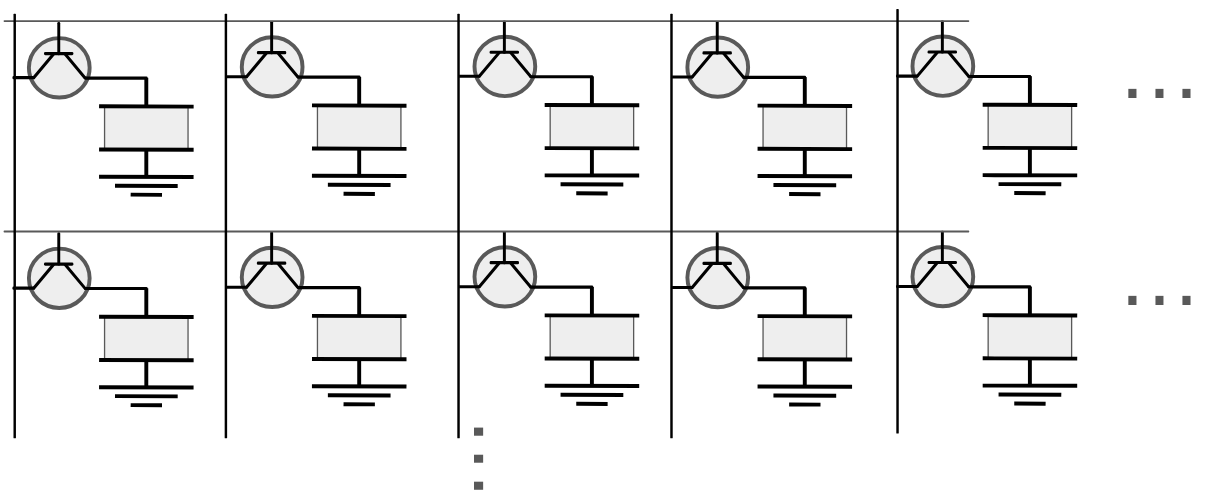
\includegraphics[scale=0.5]{assets/dram_arr.png}

  \caption{A DRAM Array.}
  \label{fig:dram-array}
\end{figure}
We can chain the individual bit storage mechanisms together to form word lines and group those together to form the full DRAM array as shown in figure~\ref{fig:dram-array}. Now that we have the full DRAM array, we can discuss filling it with data.

There are three basic operations required to perform a read on our DRAM array:
\begin{enumerate}
  \item Precharge - We apply a current with potential difference of about $0.5 * V_{full}$ to the bit lines, where $V_{full}$ is the Voltage of a full capacitor in a positive voltage system.
  \item Open the gates - Apply a current to the gates, allowing the current to flow out of the capacitors.
  \item Write back - We rewrite the data to the DRAM array.
\end{enumerate}

More detail is shown in the slide show accompanying this report.

\section{Storing a Single Bit (Static RAM)}

Static Random Access Memory (SRAM) is a type of volatile memory that stores data using bistable latching circuitry, typically made from transistors. Unlike Dynamic RAM (DRAM), which requires periodic refreshing to maintain data, SRAM maintains its data as long as power is supplied, hence the term "static."

\section{SRAM Structure}

An SRAM cell is composed of six transistors arranged in a specific configuration. The most common SRAM cell uses a \textbf{six-transistor (6T)} design. This arrangement ensures that the data is stable and does not require refreshing. A 6T SRAM cell consists of the following components:

\begin{itemize}
  \item \textbf{Two cross-coupled inverters}: These form the bistable latch that holds the data, constructed of four transistors.
  \item \textbf{Two access transistors}: These transistors control the connection to the bitlines during read and write operations.
\end{itemize}

The basic structure of a 6T SRAM cell is shown in Figure~\ref{fig:sram}.

\begin{figure}
  \centering
  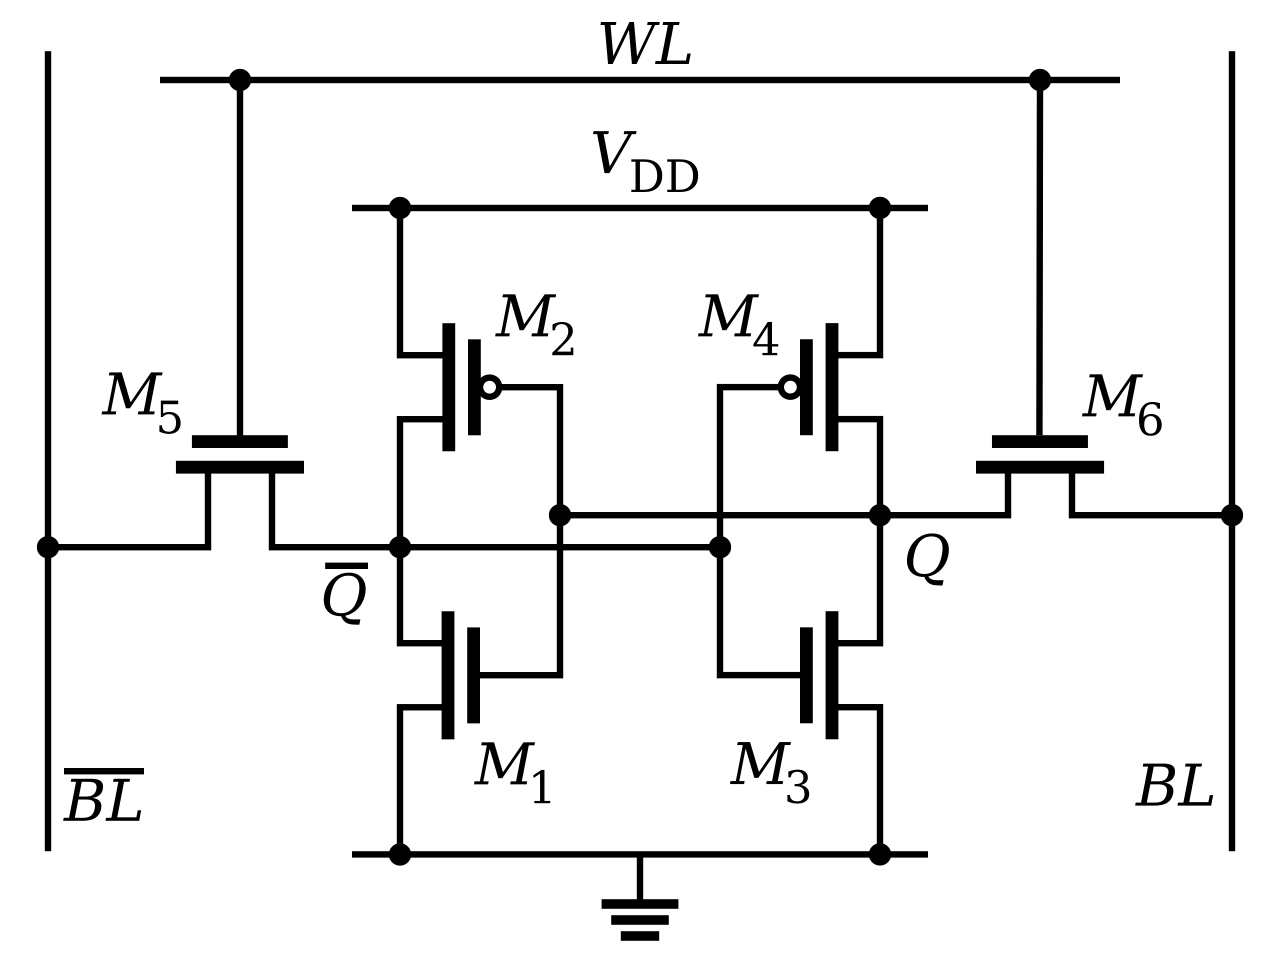
\includegraphics[scale=0.15]{assets/sram.png}
  \caption{Standard 6T SRAM Structure}
  \label{fig:sram}
\end{figure}

SRAM only differs in operation from DRAM in one step, being the final one where instead of the capacitor holding state, the cross-coupled inverters change their state. This is very similar to the operation of DRAM.

There is a different configuration that only uses four transistors. This design uses high resistance resistors with four transistors.

\begin{figure}
  \centering
  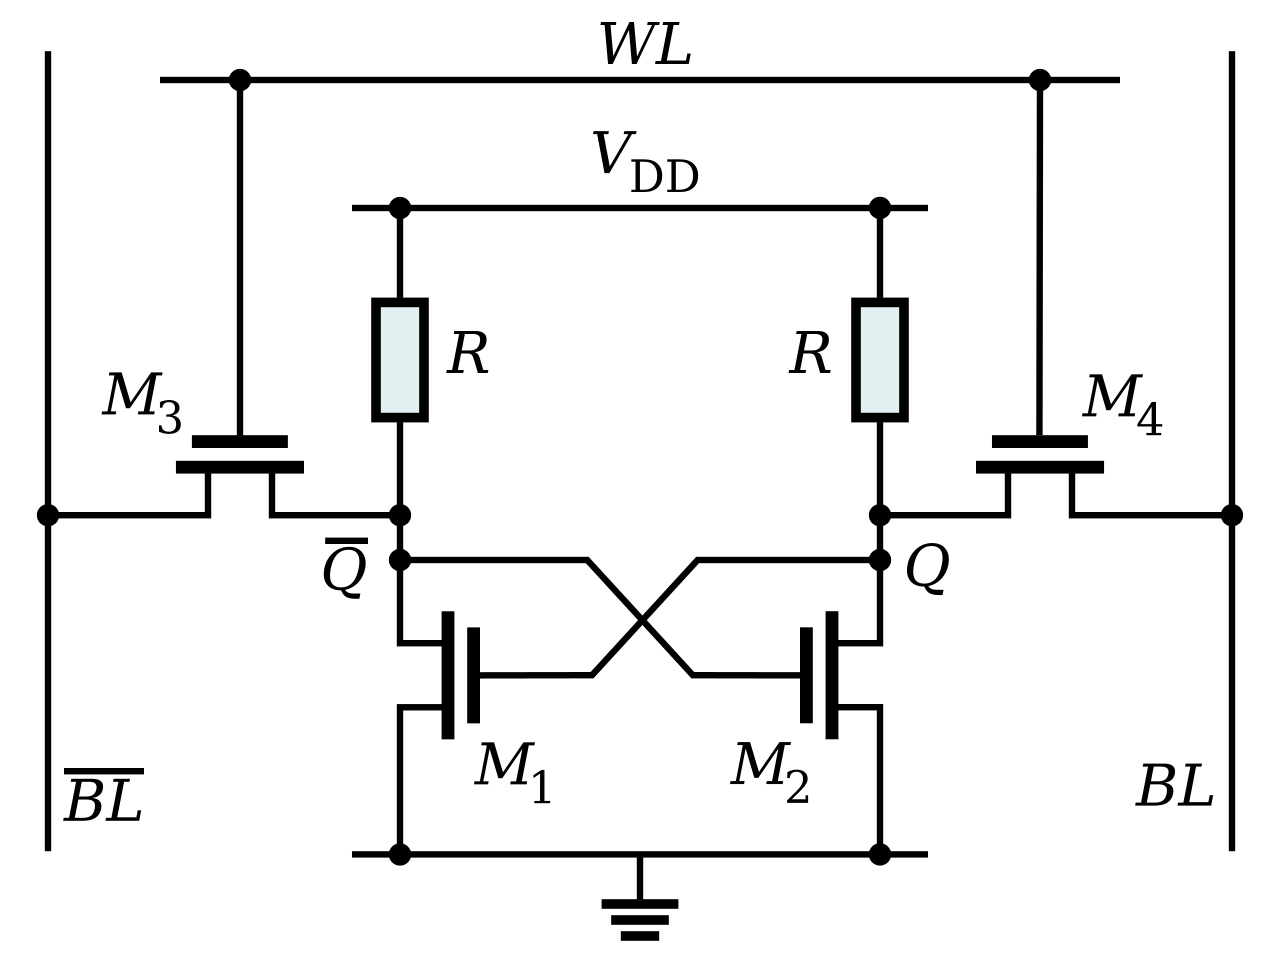
\includegraphics[scale=0.15]{assets/4tsram.png}
  \caption{Condensed 4T SRAM Structure}
  \label{fig:sram4t}
\end{figure}

\chapter{Performance Measurement in Memory}

Memory performance is based on a few key characteristics:
\begin{enumerate}
  \item Frequency
  \item CAS Latency
  \item Transfers per Second
\end{enumerate}

This leads to a few key metrics required to ensure that performance is as good as possible.

\section{Frequency}

A DRAM array has a seperate frequency from the CPU, which is synchronized with its own clock. The skew between the CPU clock and the DRAM clock is mediated by the DRAM interface. More information on the actual structure of the DRAM interface is available in~\cite{TODO}. The presence of the DRAM clock is what makes DRAM synchronous, hence SDRAM.

\section{CAS Latency}

CAS latency is a result of the time it takes for the electricity to travel through the structures of the DRAM finally resulting in the charging of the capacitor or the reading of the capacitor's charge.

%TODO how do we calculate it?

\section{Transfers per Second}

Transfers per second is directly related to the throughput of the DRAM system. The smallest data transfer you can perform across a graphics DRAM system is 32 bytes~\cite{TODO}. We can describe the total throughput of the DRAM by:
\begin{equation*}
  T_{DRAM}=k W_{interface} f_{DRAM}
\end{equation*}
where $k\in\mathbb{N}$ is the data transfer rate of the DRAM. For example, in DDR memory, we have two transfers per clock. In a normal CPU, you issue a single instruction for each clock cycle, however in DRAM you have two transfers per clock (one per clock edge). In fact, you can also do QDR which means quad data rate where you overlay two different clocks and send a signal on each clock edge.

\section{Latency in CPU Clock Cycles}

When we need to measure the overall performance of the DRAM on a CPU system, the first thing we need to consider is the time that it takes for an initial request for data to return from the DRAM. To measure this, we can use the following formula:
\begin{equation*}
  N_{cpu}=f_{cpu}(f^{-1}_{dram} CAS)
\end{equation*}
however, in a GPU system this measurement is too sensitive on latency. In a GPU system, we care significantly more about the throughput measurement than the latency due to GPU latency hiding from the warp systems.
